\section{Experiments}

\begin{figure*}
    \centering
    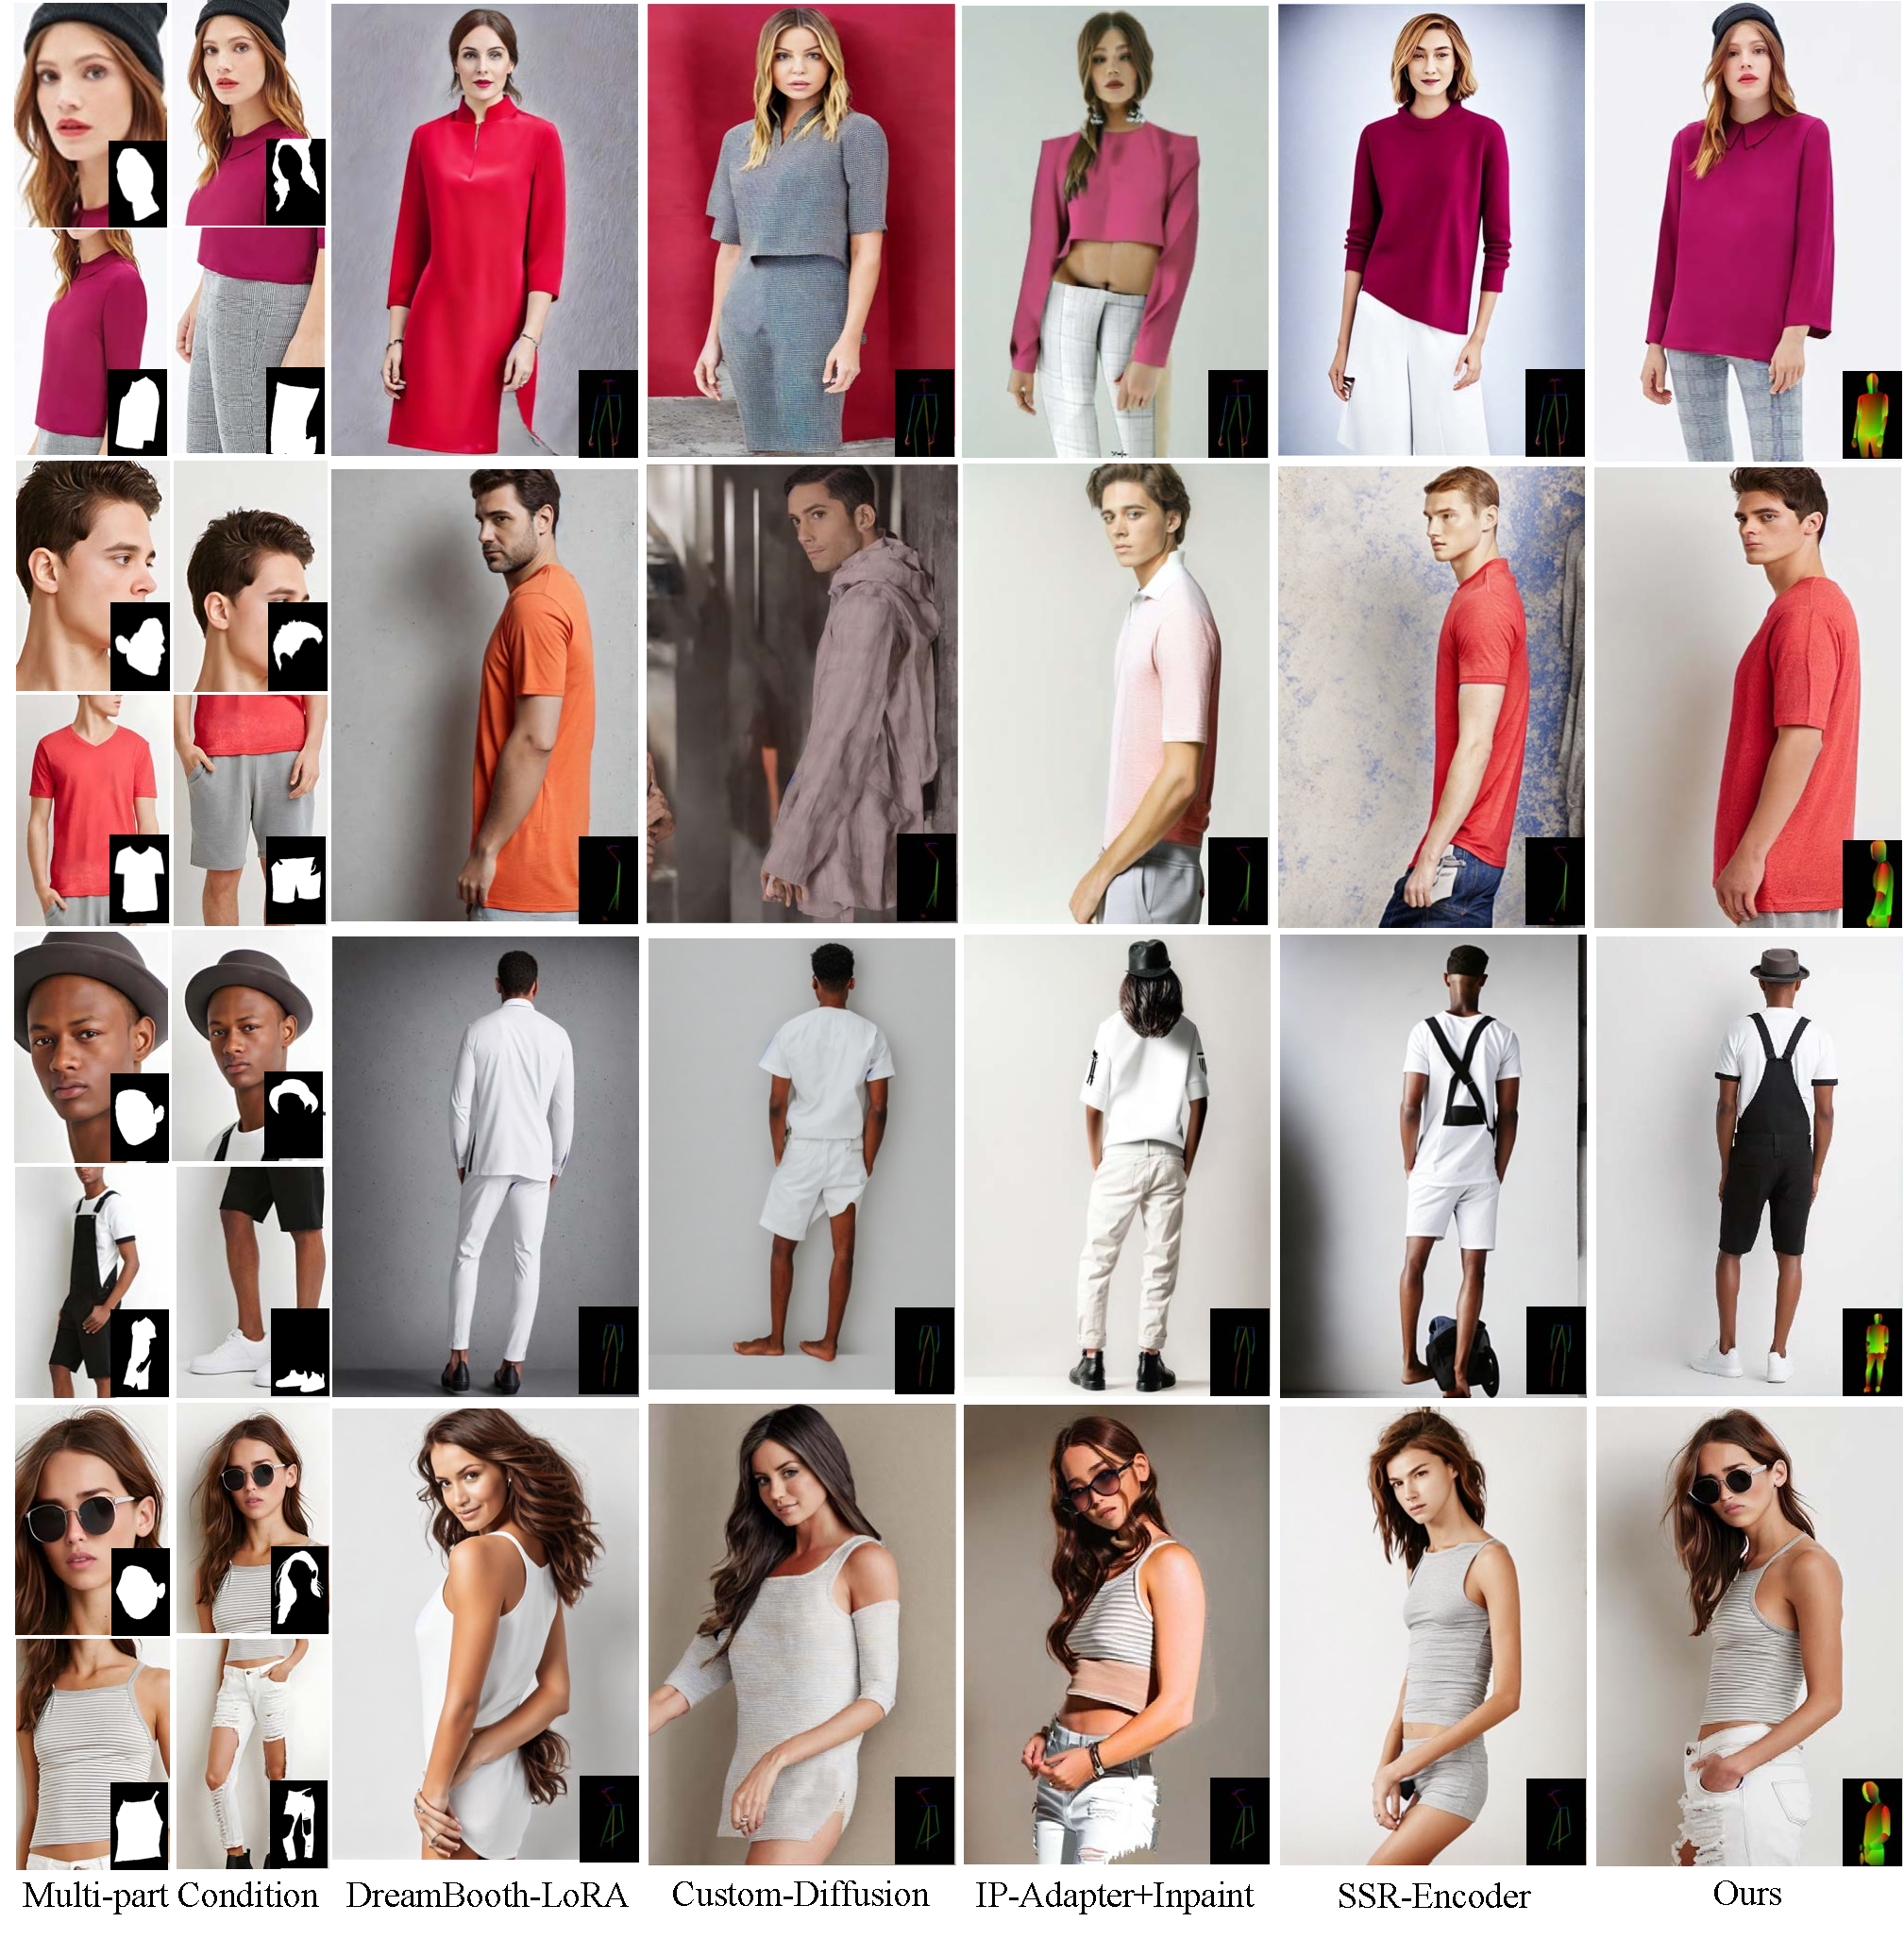
\includegraphics[width=\textwidth]{figure/comparison.pdf}
    \caption{Qualitative results generated by Parts2Whole and existing alternatives on our partitioned test set. We do not show the text condition in the figure, but notably, when we input the reference images to our proposed appearance encoder, we will pass in short labels such as face, hair or headwear, upper body clothes, lower body clothes, whole body clothes, shoes, etc.}
    \label{fig:comparison}
\end{figure*}

\subsection{Implementation Details}

\cparagraph{Dataset.}
To train the Parts2Whole model, we build a multi-modal dataset comprising about 41,500 reference-target pairs from the open-source DeepFashion-MultiModal dataset~\cite{jiang2022text2human,liuLQWTcvpr16DeepFashion}. 
Each pair in this newly constructed dataset includes multiple reference images, which encompass human pose images (e.g., OpenPose, Human Parsing, DensePose), various aspects of human appearance (e.g., hair, face, clothes, shoes) with their short textual labels, and a target image featuring the same individual (ID) in the same outfit but in a different pose, along with textual captions.

The DeepFashion-MultiModal dataset exhibits noise in its ID data. For example, different images tagged with the same ID but depicting different individuals. To address this issue, we first cleanse the IDs by extracting facial ID features from images tagged with the same ID using InsightFace\cite{deng2018arcface, InsightFaceProject}. Cosine similarity is then used to evaluate the similarity between image ID feature pairs to distinguish between different ID images within the same ID group. Subsequently, we utilize DWPose\cite{yang2023dwpose} to generate pose images corresponding to each image. Guided by human parsing files, we crop human images into various parts. Due to the low resolution of the cropped parts, we apply Real-ESRGAN\cite{wang2021realesrgan} to enhance the image resolution, thus obtaining clearer reference images. Textual descriptions of the original dataset are used as captions. For constructing pairs, we select images with cleaned IDs that feature the same clothes and individual but in different poses. Specifically, a pair contains multiple parts from one human image as reference images, and an image of the person in another pose as the target. Finally, we build a total of about 41,500 pairs, of which the training set is about 40,000 and the test set is about 1,500 pairs.

\cparagraph{Detailed Configurations.}
In this work, the denoising U-Net and the appearance encoder both leverage the pre-trained weights from Stable Diffusion-1.5~\cite{rombach2022ldm}. We use CLIP Vision Model with projection layers as our image encoder, initialized with Stable Diffusion Image Variations~\cite{sdimagevariation}. During training, we set the initial learning rate 1e-5 with a batch size of 64. The models are trained using 8 NVIDIA A800 GPUs, for a total of 30000 iterations. To maintain the capability and generalizability of image generation, we randomly drop all of the reference image features and the pose condition with a probability of 0.2. At the same time, to improve the flexibility of generation, we randomly drop each appearance condition with a probability of 0.2, so that the portrait generation can be conditioned on indefinite reference images. In the inference stage, we adopt DDIM sampler~\cite{song2020ddim} with 50 steps, and set the guidance scale to 7.5.

\subsection{Comparison with Existing Alternatives}

Our Parts2Whole targets at controllable human image generation conditioned on multiple parts of human appearance. To evaluate the performance of our proposed framework, we compare our Parts2Whole with existing subject-driven solutions. For fairness, we make some improvements to the methods, to make them more suitable for generating human images from multiple conditions.

\cparagraph{Test-time Fine-tuning Methods.}
Among the tuning-based methods, we adopt DreamBooth LoRA~\cite{ruiz2023dreambooth,hu2021lora} and Custom Diffusion~\cite{kumari2023customdiffusion} as baseline methods for comparison, as these methods are relatively robust and effective. DreamBooth LoRA inserts a smaller number of new weights into Stable Diffusion~\cite{rombach2022ldm} and only trains these parameters on just a few images of a subject or style, thereby associating a special word in the prompt with the example images. Custom Diffusion fine-tunes only key and value projection matrices in the cross-attention layers, to customize text-to-image models. Given as input several aspects of human appearance, we use these two methods to fine-tune Stable Diffusion, such that it learns to bind identifiers with specific human parts. As shown in Fig.~\ref{fig:comparison}, when it comes to multi-aspect composition, the attributes of different parts in images generated by these tuning-base methods mix together, resulting in unrealistic human images. In contrast, Parts2Whole generates high-fidelity results without the need for parameter tuning.

\cparagraph{Reference-based Methods.}
Among the tuning-free methods, we adopt IP-Adapter~\cite{ye2023ipadapter} and SSR-Encoder~\cite{zhang2024ssrencoder} for comparison. IP-Adapter is an image prompt adapter that can be plugged into diffusion models to enable image prompting, and can be combined with other adapters like ControlNet~\cite{zhang2023controlnet}. We firstly use IP-Adapter FaceID and ControlNet to generate human images from facial appearance and pose maps. Then we repaint hair, clothes, shoes and other areas using the specific image step by step, thereby achieving multi-image conditioned generation of portraits in a multi-step way. SSR-Encoder is an effective encoder designed for selectively capturing any subject from single or multiple reference images by the text query or mask query. For fairness, we fine-tune it in our human dataset to enhance its ability for human images.

We compare our Parts2Whole with the above two reference-based alternatives in the test set. For quantitative comparison, we compute the commonly used CLIP score and DINO score to evaluate the similarity between the generated image and the specified human parts. For further alignment evaluation, we use DreamSim~\cite{fu2023dreamsim}, a new metric for perceptual image similarity that bridges the gap between "low-level" metrics (e.g. LPIPS, PSNR, SSIM) and "high-level" measures (e.g. CLIP). Since the generated image is conditioned on multiple parts of human appearance, it is difficult to evaluate the degree of alignment by calculating the average metric with these multiple images. Therefore, we calculate the above three indicators between the output image and the original reference portrait from which these different parts come. We present the quantitative results in Tab.~\ref{tab:quan_comp} and the qualitative results in Fig.~\ref{fig:comparison}. Both IP-Adapter and SSR-Encoder fails to maintain alignment with the specified appearance images and often produce unrealistic results when multi-part combinations are involved. In comparison, our method achieves the best results in terms of image quality and appearance alignment.

\begin{table}\small
  \centering
  \caption{Quantitative comparison between our Parts2Whole and existing reference-based alternatives.}
  \begin{tabular}{@{}lccc@{}}
    \toprule
    Method & CLIP$\uparrow$ & DINO$\uparrow$ & DreamSim\cite{fu2023dreamsim}$\downarrow$ \\
    \midrule
    IP-Adapter~\cite{ye2023ipadapter} + Inpaint & 80.1 & 69.8 & 0.445   \\
    SSR-Encoder~\cite{zhang2024ssrencoder} & 86.9 & 75.1 & 0.346 \\
   Parts2Whole (Ours) & \textbf{91.2} & \textbf{93.7} & \textbf{0.221}  \\
    \bottomrule
  \end{tabular}
  \label{tab:quan_comp}
\end{table}

\cparagraph{User Study.}
We conduct a user study to further evaluate the reference-based methods IP-Adapter~\cite{ye2023ipadapter}, SSR-Encoder~\cite{zhang2024ssrencoder} and our Parts2Whole. We randomly select 20 pairs of reference-target pairs from the test set. For each pair, we provide multiple referential appearance images, pose images, textual captions and the generated human images. We evaluate the performance from two main aspects: first, the \textbf{quality} of the generated images, where quality primarily refers to the realism, rationality, and clarity of the images; and second, the \textbf{similarity} between the generated images and the reference images. The similarity assessment includes consistency in ID, pose, texture, color, and style between the generated images and the reference images. We involve 20 users in the user study, who are required to score the three methods based on these two evaluative aspects. The final experimental results are shown in Tab.~\ref{tab:user_study}, from which we observe that our model owns obvious superiorities for alignment with given appearance conditions.

\begin{table}
  \centering
  \caption{User study on the comparison with existing reference-based alternatives. "Quality" and "Similarity" measures synthesis quality and appearance preservation. Each metric is rated from 1 (worst) to 5 (best).}
  \begin{tabular}{@{}lcccc@{}}
    \toprule
    Method & Quality$\uparrow$ & Similarity$\uparrow$ \\
    \midrule
    IP-Adapter~\cite{ye2023ipadapter} + Inpaint &  3.78 & 3.58  \\
    SSR-Encoder~\cite{zhang2024ssrencoder} & 3.64  & 3.14 \\
   Parts2Whole (Ours) & \textbf{4.52} & \textbf{4.55} \\
    \bottomrule
  \end{tabular}
  \label{tab:user_study}
\end{table}

\subsection{Ablation Studies}

\begin{figure*}
    \centering
    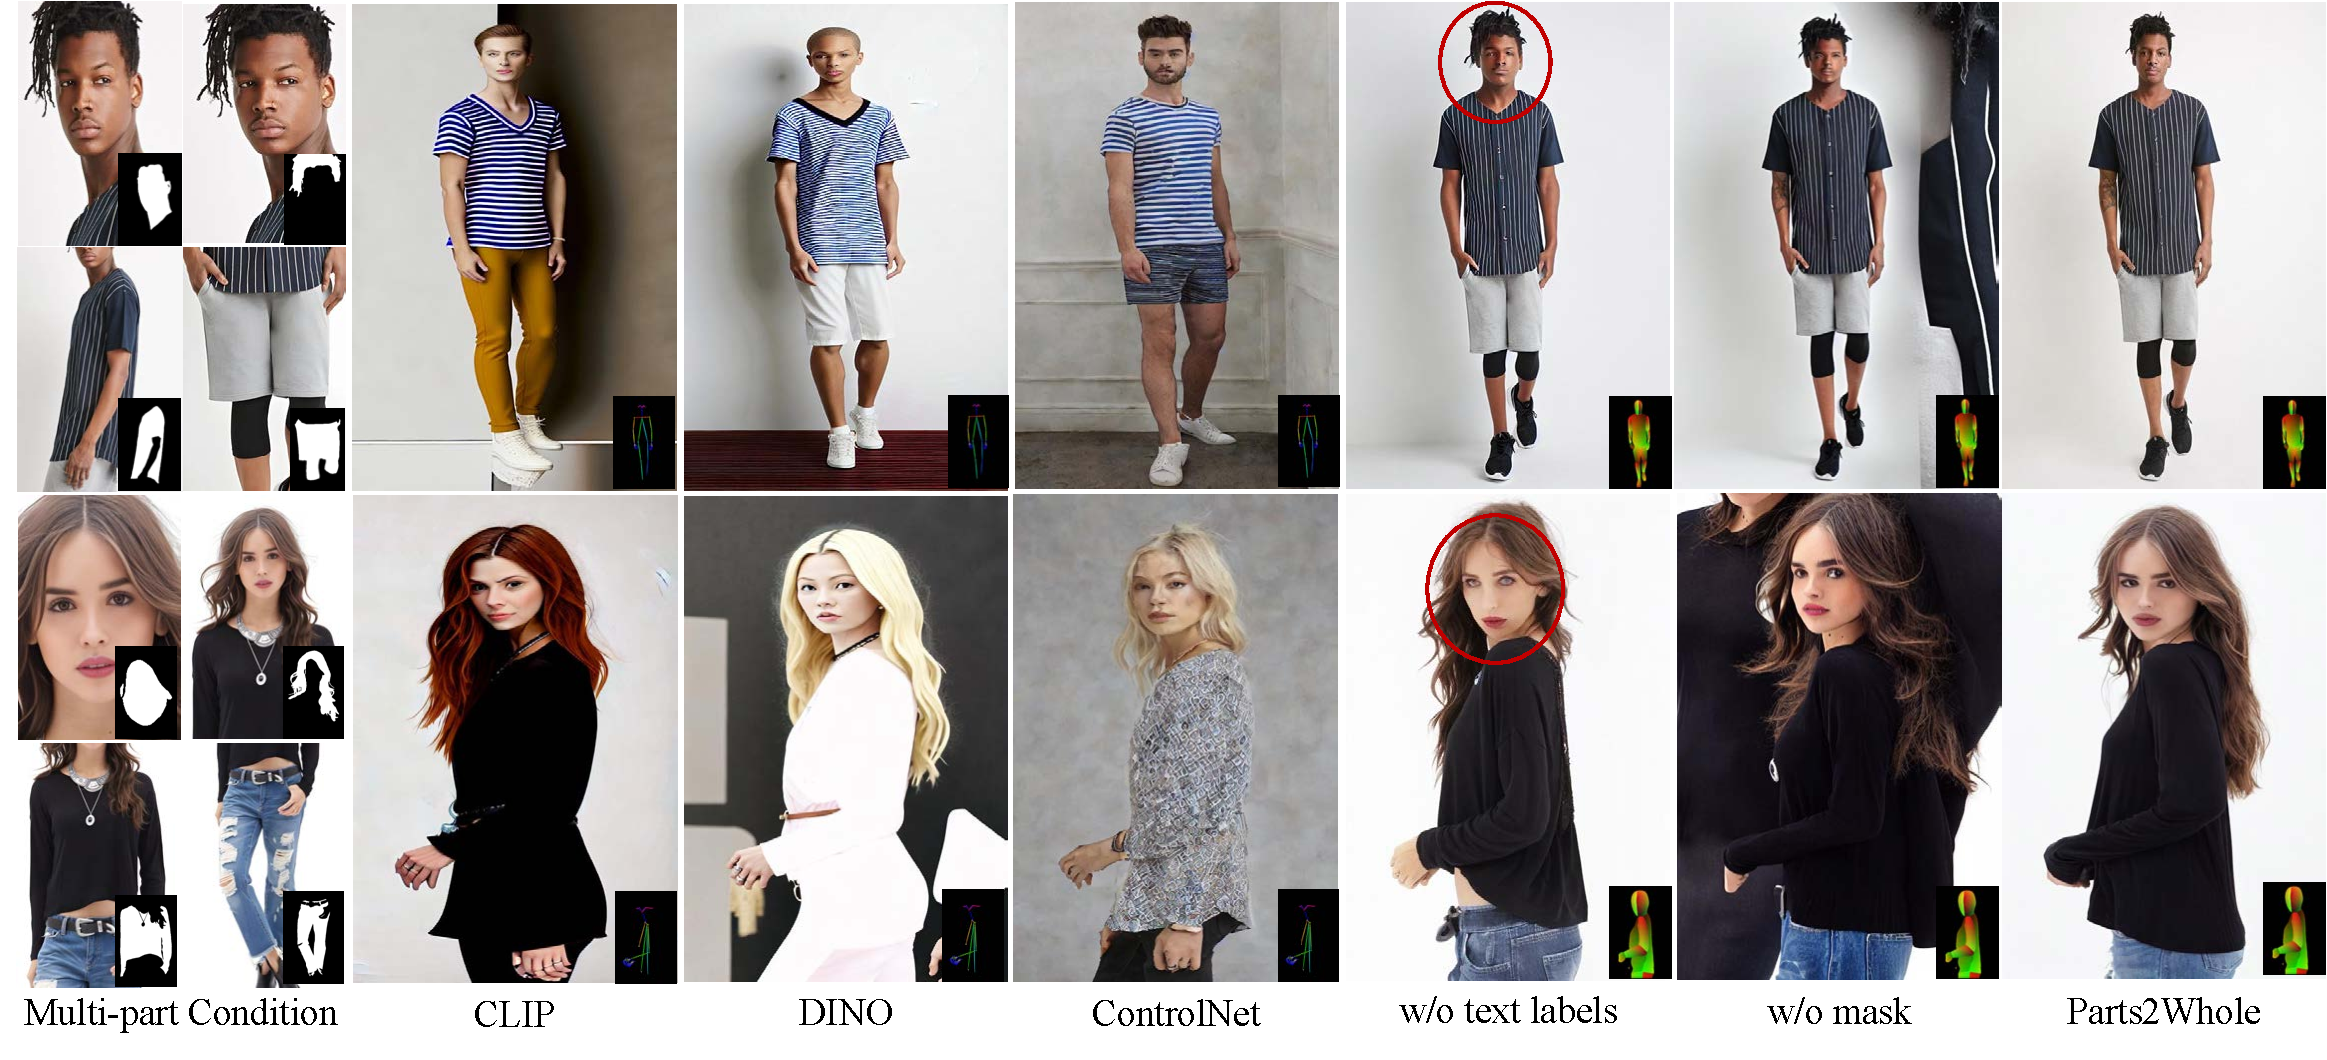
\includegraphics[width=\textwidth]{figure/ablation.pdf}
    \caption{Qualitative analysis of using different backbones for the appearance encoder, and our proposed methods.}
    \label{fig:ablation}
\end{figure*}

\cparagraph{Appearance Encoder for Multiple Images.}
As described in Sec.~\ref{subsec:unifiedref}, to extract detailed features from multiple reference images, our Parts2Whole designs an appearance encoder by copying the network structure and pre-trained weights from the denoising U-Net. Here, we compare it to the baseline with other image encoders. Specifically, we leverage the CLIP image encoder~\cite{radford2021clip}, DINOv2~\cite{oquab2024dinov2}, and ControlNet~\cite{zhang2023controlnet} as feature extractors and apply the same training settings for fair comparison. The qualitative results of generated human images are presented in Fig.~\ref{fig:ablation}. From the second and third columns of the figure, we observe that these semantic-level feature extractors cannot preserve the appearance details of multiple reference images and only extract color and rough texture. ControlNet directly adds different image features with misaligned structures to the feature maps, resulting in unstable image quality. In contrast, our preposed appearance encoder provides fine-grained details of multiple aspects of human appearance.

\cparagraph{Semantic-Aware Encoder.} In the process of encoding multiple reference image features, we provide a textual class label for each aspect of human appearance, thus providing a classifier-like guidance. To assess the effectiveness of the additional external condition, we compare it with directly concatenating multiple reference images in the dimension of width as input to the appearance encoder. As shown in the 5th column in Fig.~\ref{fig:ablation}, simply piecing reference images can also produce images relatively aligned with the given images, but leads to stiff-looking and unrealistic results. This is because modeling only the image itself makes the model lack awareness of different types of appearances. Conversely, after injecting different semantic labels for each reference image, the model has awareness of various parts of the human appearance, producing realistic and flexible portraits.

\cparagraph{Mask-Guided Subject Selection.}
To precisely select subjects from multiple reference images, we introduce the subject masks into the shared self-attention mechanism. To evaluate the effectiveness of our proposed mask-guided attention, we compare it with that without masks. The visualization results can be found in the 6th column of Fig.~\ref{fig:ablation}. When not using subject masks, the image is generated with reference to all patches of the conditional images, including the unexpected background or other parts. Due to the generation being interfered with by irrelevant subjects, the model produces homogeneous colors or appears with unexpected background or subjects. On the contrary, with the support of mask-guided attention, Parts2Whole accurately refers to the appearance of the specified parts to generate real human images.

\begin{table}\small
  \centering
  \caption{Quantitative analysis of using semantic-aware encoder and mask-guided subject selection.}
  \begin{tabular}{@{}lcccc@{}}
    \toprule
    Method & CLIP$\uparrow$ & DINO$\uparrow$ & DreamSim\cite{fu2023dreamsim}$\downarrow$ & FID$\downarrow$ \\
    \midrule
    w/o text labels & 90.1 & 91.9 & 0.248 & 23.95 \\
    w/o mask & 90.8 & 91.6 & 0.243 & 19.79 \\
   Parts2Whole & \textbf{91.2} & \textbf{93.7} & \textbf{0.221} & \textbf{17.29} \\
    \bottomrule
  \end{tabular}
  \label{tab:abla}
\end{table}
